
\documentclass[border=1pt, crop, multi, tikz]{standalone} 
\usepackage{import}
\subimport{/home/thesis/PlotNeuralNets/layers/}{init}
\usetikzlibrary{positioning}
\usetikzlibrary{3d} %for including external image 


\def\ConvColor{rgb:yellow,5;red,2.5;white,5}
\def\ConvReluColor{rgb:yellow,5;red,5;white,5}
\def\PoolColor{rgb:red,1;black,0.3}
\def\UnpoolColor{rgb:blue,2;green,1;black,0.3}
\def\FcColor{rgb:blue,5;red,2.5;white,5}
\def\FcReluColor{rgb:blue,5;red,5;white,4}
\def\SoftmaxColor{rgb:magenta,5;black,7}   
\def\SumColor{rgb:blue,5;green,15}


\newcommand{\copymidarrow}{\tikz \draw[-Stealth,line width=0.8mm,draw={rgb:blue,4;red,1;green,1;black,3}] (-0.3,0) -- ++(0.3,0);}

\begin{document}
\begin{tikzpicture}
\tikzstyle{connection}=[ultra thick,every node/.style={sloped,allow upside down},draw=\edgecolor,opacity=0.7]
\tikzstyle{copyconnection}=[ultra thick,every node/.style={sloped,allow upside down},draw={rgb:blue,4;red,1;green,1;black,3},opacity=0.7]


\node[canvas is zy plane at x=0] (input) at (-3,0,0) {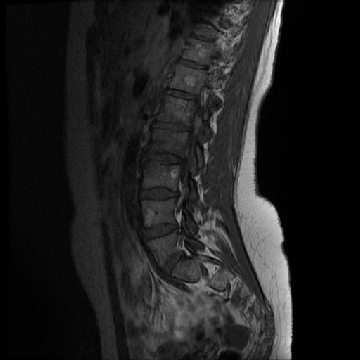
\includegraphics[width=10.0cm,height=10.0cm]{/home/thesis/PlotNeuralNets/images/input.png}};


\pic[shift={ (0,0,0) }] at (0,0,0) 
    {RightBandedBox={
        name=cr1,
        caption=conv1,
        xlabel={{ 64,64 }},
        zlabel=352,
        fill=\ConvColor,
        bandfill=\ConvReluColor,
        height=40,
        width={ 2,2 },
        depth=40
        }
    };


\pic[shift={ (0,0,0) }] at (cr1-east) 
    {Box={
        name=p1,
        caption= ,
        fill=\PoolColor,
        opacity=0.5,
        height=35,
        width=1,
        depth=35
        }
    };


\pic[shift={ (1,0,0) }] at (p1-east) 
    {RightBandedBox={
        name=cr2,
        caption=conv2,
        xlabel={{ 128,128 }},
        zlabel=128,
        fill=\ConvColor,
        bandfill=\ConvReluColor,
        height=35,
        width={ 4,4 },
        depth=35
        }
    };


\pic[shift={ (0,0,0) }] at (cr2-east) 
    {Box={
        name=p2,
        caption= ,
        fill=\PoolColor,
        opacity=0.5,
        height=30,
        width=1,
        depth=30
        }
    };


\pic[shift={ (1,0,0) }] at (p2-east) 
    {RightBandedBox={
        name=cr3,
        caption=conv3,
        xlabel={{ 256,256,256 }},
        zlabel=64,
        fill=\ConvColor,
        bandfill=\ConvReluColor,
        height=30,
        width={ 4,4,4 },
        depth=30
        }
    };


\pic[shift={ (0,0,0) }] at (cr3-east) 
    {Box={
        name=p3,
        caption= ,
        fill=\PoolColor,
        opacity=0.5,
        height=23,
        width=1,
        depth=23
        }
    };


\pic[shift={ (1,0,0) }] at (p3-east) 
    {RightBandedBox={
        name=cr4,
        caption=conv4,
        xlabel={{ 512,512,512 }},
        zlabel=32,
        fill=\ConvColor,
        bandfill=\ConvReluColor,
        height=23,
        width={ 4,4,4 },
        depth=23
        }
    };


\pic[shift={ (0,0,0) }] at (cr4-east) 
    {Box={
        name=p4,
        caption= ,
        fill=\PoolColor,
        opacity=0.5,
        height=15,
        width=1,
        depth=15
        }
    };


\pic[shift={ (1,0,0) }] at (p4-east) 
    {RightBandedBox={
        name=cr5,
        caption=conv5,
        xlabel={{ 512,512,512 }},
        zlabel=16,
        fill=\ConvColor,
        bandfill=\ConvReluColor,
        height=15,
        width={ 4,4,4 },
        depth=15
        }
    };


\pic[shift={ (0,0,0) }] at (cr5-east) 
    {Box={
        name=p5,
        caption= ,
        fill=\PoolColor,
        opacity=0.5,
        height=10,
        width=1,
        depth=10
        }
    };


\pic[shift={ (1,0,0) }] at (p5-east) 
    {RightBandedBox={
        name=fc7,
        caption=conv6,
        xlabel={{ 4096,4096 }},
        zlabel=16,
        fill=\ConvColor,
        bandfill=\ConvReluColor,
        height=15,
        width={ 6,6 },
        depth=15
        }
    };


\pic[shift={(1,0,0)}] at (fc7-east) 
    {Box={
        name=score,
        caption=scoring,
        xlabel={{6, }},
        zlabel=16,
        fill=\ConvColor,
        height=15,
        width=1,
        depth=15
        }
    };


\pic[shift={ (0.5,-10,0) }] at (p3-east) 
    {RightBandedBox={
        name=up3,
        caption= ,
        xlabel={{ 6, }},
        zlabel=352,
        fill={rgb:white,1;black,3},
        bandfill={rgb:white,1;black,2},
        opacity=0.5,
        height=35,
        width=1,
        depth=35
        }
    };


\pic[shift={(1,0,0)}] at (up3-east) 
    {Ball={
        name=s3,
        fill=\SumColor,
        opacity=0.6,
        radius=2.5,
        logo=$+$
        }
    };


\pic[shift={ (0.5,-10,0) }] at (p4-east) 
    {RightBandedBox={
        name=up4,
        caption= ,
        xlabel={{ 6, }},
        zlabel=352,
        fill={rgb:white,1;black,3},
        bandfill={rgb:white,1;black,2},
        opacity=0.5,
        height=35,
        width=1,
        depth=35
        }
    };


\pic[shift={(2,0,0)}] at (up4-east) 
    {Ball={
        name=s4,
        fill=\SumColor,
        opacity=0.6,
        radius=2.5,
        logo=$+$
        }
    };


\pic[shift={ (0.5,-10,0) }] at (score-east) 
    {RightBandedBox={
        name=up7,
        caption= ,
        xlabel={{ 6, }},
        zlabel=352,
        fill={rgb:white,1;black,3},
        bandfill={rgb:white,1;black,2},
        opacity=0.5,
        height=35,
        width=1,
        depth=35
        }
    };


\draw [connection]  (p1-east)    -- node {\midarrow} (cr2-west); % end to_connection


\draw [connection]  (p2-east)    -- node {\midarrow} (cr3-west); % end to_connection


\draw [connection]  (p3-east)    -- node {\midarrow} (cr4-west); % end to_connection


\draw [connection]  (p4-east)    -- node {\midarrow} (cr5-west); % end to_connection


\draw [connection]  (p5-east)    -- node {\midarrow} (fc7-west); % end to_connection


\draw [connection]  (p3-east)    -- node {\midarrow} (up3-west); % end to_connection


\draw [connection]  (up3-east)    -- node {\midarrow} (s3-west); % end to_connection


\draw [connection]  (s3-east)    -- node {\midarrow} (up4-west); % end to_connection


\draw [connection]  (p4-east)    -- node {\midarrow} (up4-west); % end to_connection


\draw [connection]  (up4-east)    -- node {\midarrow} (s4-west); % end to_connection


\draw [connection]  (s4-east)    -- node {\midarrow} (up7-west); % end to_connection


\draw [connection]  (fc7-east)    -- node {\midarrow} (score-west); % end to_connection


\draw [connection]  (score-east)    -- node {\midarrow} (up7-west); % end to_connection


\end{tikzpicture}
\end{document}

